\documentclass[12pt]{beamer}

\usepackage{ucs}
\usepackage[utf8x]{inputenc}
\usepackage{beamerthemeBerkeley}

\usepackage[australian]{babel}
\usepackage[T1]{fontenc}
\usepackage{graphicx}

\title{PODD Ontology Driven Database}
\author{Dr Peter Ansell}
\institute{University of Queensland}
\date{13 March 2012}

\begin{document}

\begin{frame}
\titlepage
\end{frame}

\begin{frame}{Outline}
  \tableofcontents
  % You might wish to add the option [pausesections]
\end{frame}

\section{Scientific experiments}

\begin{frame}
\frametitle{Scientific experiments}

\begin{itemize}
 \item Aim to test hypotheses in known, partially controlled, situations
\pause
 \item Contain many variables
\pause
 \item Experiment variables and results are noted and used in analysis
\pause
 \item Analysed results are used to make conclusions, which are then published
\end{itemize}
\end{frame}

\begin{frame}
\frametitle{Scientific workbooks}

\begin{itemize}
 \item Some common headings
\pause
 \item Structure can vary
\end{itemize}
\end{frame}

\section{Structured data}

\begin{frame}
\frametitle{Relational databases}

\begin{itemize}
 \item Two dimensional structure
\pause
 \item Suit simple relationships
\pause
 \item Single table not ideal for entire experiment
\pause
 \item Not ideal for multiple structurally different experiments
\end{itemize}
\end{frame}

\begin{frame}
\frametitle{Structured ontologies}

\begin{itemize}
 \item A common root
\pause
 \item Branches and leaves are independent of each other
\end{itemize}
\end{frame}

\section{PODD Ontology Driven Database}

\begin{frame}
\frametitle{PODD as a workbook}

\begin{itemize}
 \item Vital metadata about each experiment in a single ontology
\pause
 \item Variable number of headings and subheadings
\pause
 \item Acceptable use of headings and subheadings is configurable
\pause
 \item Each experiment is independent of other experiments
\end{itemize}
\end{frame}

\begin{frame}
\frametitle{Ontologies to define structure}

\begin{itemize}
 \item Different structures for different experiments without changing the database schema
\pause
 \item PODD has basic ontology constraints
\begin{enumerate}
 \item Each ontology must have exactly one Project
 \item Each node must be connected to the Project through a unique series of ``part\_of'' links
 \item Each node can reference other eligible nodes using ``refers\_to'' links
\end{enumerate}
\pause
\item A single ontology can be used with different experiments if it is designed well
\end{itemize}
\end{frame}

\begin{frame}
\frametitle{Phenomics ontology structure}

\begin{center}
 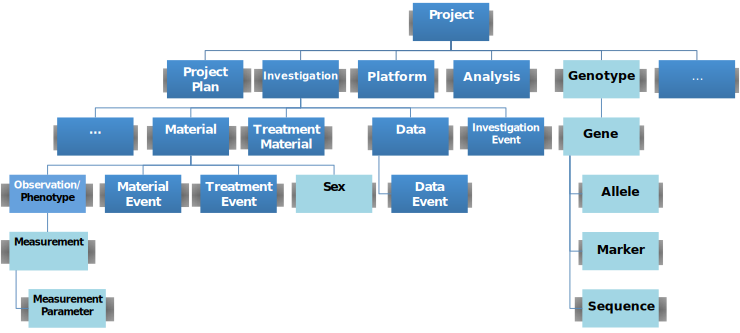
\includegraphics[scale=0.36,keepaspectratio=true]{./podd_ont.pdf}
 % podd_ont.pdf: 720x540 pixel, 72dpi, 25.40x19.05 cm, bb=0 0 720 540
\end{center}
\end{frame}

\begin{frame}
\frametitle{Publication}

\begin{itemize}
 \item Projects can be published on completion, both in HTML and RDF
\pause
 \item Published projects may be locked from future changes
\pause
 \item Each data item has a URI for references
\end{itemize}
\end{frame}

\begin{frame}
\frametitle{Questions}

Code can be found online at:

\url{https://github.com/podd}

\end{frame}

\end{document}


